\documentclass[UTF8]{book}
\usepackage{graphicx}
\usepackage{caption}
\usepackage{subcaption}
\usepackage{float}
\usepackage{amsmath}
\usepackage{seqsplit}
\usepackage{tikz}
\usepackage{pgfplots}
\usepackage{listings}
\usepackage{CJK}

\newtheorem{theorem}{Proposition}
\newcommand\longnumber[2]{%
    \begin{minipage}{#1}
    \seqsplit{#2}
    \end{minipage}
    }
\newcommand*\thickdash{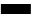
\includegraphics{thick-dash2}}
\newcommand*\thickdot{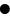
\includegraphics{thick-dot2}}

\graphicspath{ {images/} }
\begin{document}
\begin{CJK}{UTF8}{gbsn}

\title{The Network}
\author{Dan Auerbach}
\date{2015}
\maketitle


\part{The Telegraph}

\chapter{Communication at a Distance}

The electrical telegraph brought near-instantaneous communication to the Victorian world in the mid 1800s, accelerating commerce, business and establishing the magical transformative power of electricity. Yet long before telegraph engineers were plotting spider webs of wires connecting the world's cities, the word ``telegraph'' was already in widespread use. Much like signal fires in use since antiquity to convey simple yes-or-no messages, this \emph{optical telegraph} required no wires at all, instead relying on ordinary sight.

\section{Telecommunications Using Plain Sight}

Suppose you decide to play a game of catch with your friend Mary. After throwing back and forth a little, the inner athlete in Mary takes over and she decides just throwing the ball around is too boring -- she wants to practice some drills.

You're too far apart to yell at each other, so she waves you over. Soon she is excitedly describing her workout plan to you: for each throw, she is going to tell you whether she wants a high ball or a fast line drive ball thrown hard, and your job is to deliver these balls. The point of the exercise is not to surprise her -- she prefers to know what is coming -- but rather to deliver the throws she wants as accurately as possible.

You grumble to yourself about Mary's inability to just have fun without making activities so competitive, but know that it would be futile to resist. And besides, you have a much more practical question in front of you: how is she going to indicate if she wants a high ball or a low ball? You are not in shouting distance. You briefly consider having her hold up one finger for a high ball, and two for a low ball, but quickly realize it will be hard to discern the number of fingers she's holding up from a distance.

Then you figure out a system that works. She will raise her right arm straight up in indicate that she wants a high ball thrown, and will put her right arm straight out sideways for a low ball:

\begin{figure}[H]
\centering
\captionsetup{labelformat=empty}
\begin{minipage}{.4\textwidth}
  \centering
  
\includegraphics[width=.3\linewidth]{stick-figure-arm-raised}
  \captionof{figure}{High ball}
  \label{fig:test1}
\end{minipage}%
\begin{minipage}{.4\textwidth}
  \centering
  
\includegraphics[width=.3\linewidth]{stick-figure-arm-sideways}
  \captionof{figure}{Low ball}
  \label{fig:test2}
\end{minipage}
\end{figure}

This works like a charm. Mary chooses the ball she wants, and gets to practice her catching, and you have to admit that it is kind of fun to practice particular types of throws instead of just generally playing catch.

Now, just as you are getting into a rhythm, Mary waves you over again. Uh oh. Your suspicions are quickly vindicated as she explains that she now wants to be able to signal one of \emph{six} different types of throws for you to deliver to her. After some grumbling, you give in and find yourself again faced with the task of coming up with a system for distinguishing the throws from one another without being able to communicate verbally.

The arm-based signaling system was working pretty well, so you decide to extend it, this time using two arms instead of one:

\begin{figure}[H]
\centering

\includegraphics{stick-figure-six-positions-simplified}
\end{figure}

It takes a little getting used to, but you pick up the system and once again settle into a rhythm, having hopefully satiated your throwing partner's lust for pushing her body to the limit. Your mind wanders, and you start thinking about the system you just devised. Can it be extended further? Is there a limit to how much information you can convey with just two arms?

After thinking through it a bit more, you realize that if you could represent every letter of the alphabet via a different set of arm positions, then by using your arm positions to represent individual letters, one at a time, you could communicate entire sentences via through arm positions alone:

\begin{figure}[H]
\centering
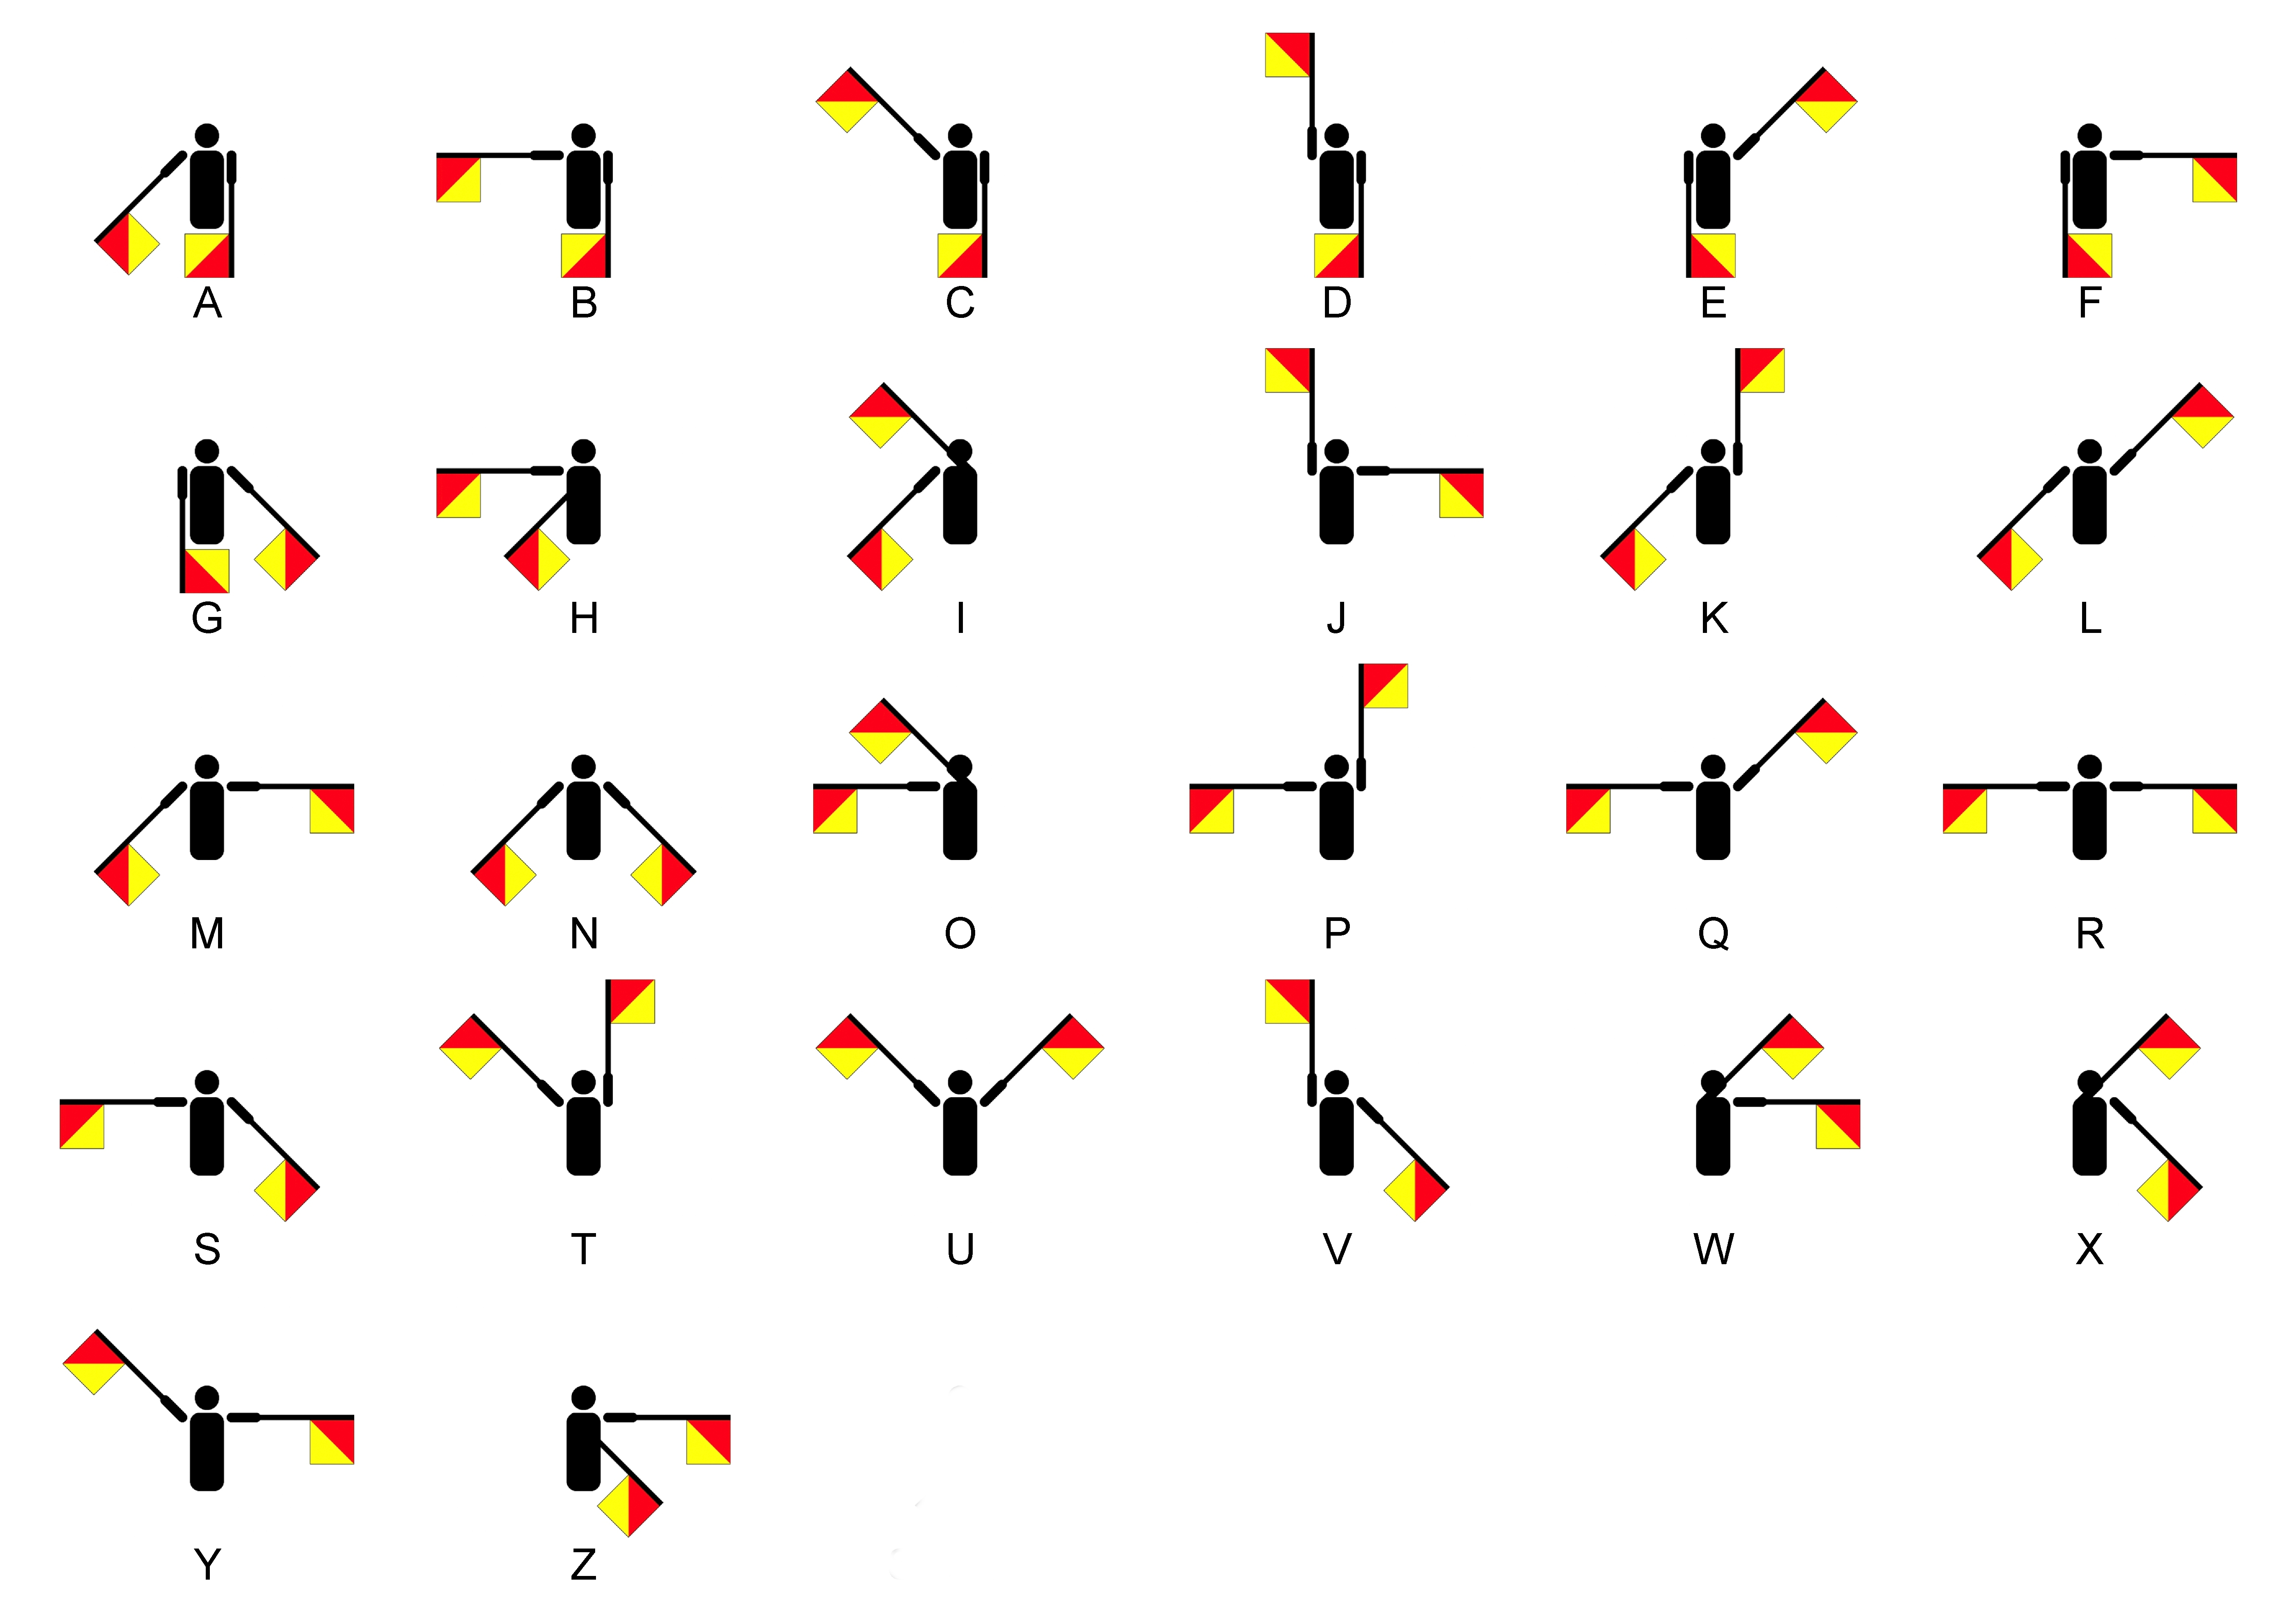
\includegraphics[width=0.9\linewidth]{semaphoreflags3}
\end{figure}

Here we display one possible system where the person signaling holds flags for extra emphasis so that the arm positions can be seen from far away.

Using this system, you could compose a message (``hey Mary, let's stop being so intense when we play catch''), and pass that message to Mary one letter at a time encoded via your arm signaling system, who in turn could decode it and understand the message.

This system is an example of what is called a \emph{semaphore system} of communication. While it may not seem that groundbreaking or useful for your game of catch, this core idea of encoding useful information into symbols and then transmitting those symbols is the essence of all communication in the Internet era.

Now you might naturally wonder: is there any way for us to extend this idea to quickly transfer information across dozens or even hundreds of miles? To turn this basic semaphore system into something useful, we will need a \emph{network} of relay stations, each passing a message along to the next faster than any horse could ride.

\begin{figure}[H]
\centering

\includegraphics[width=0.9\linewidth]{relay_stations}
\end{figure}

Even those in the ancient world understood that relay stations could be used in this way to transmit visual information, and they did this through the creation of networks of signal fires. For example, the play \emph{Agamemnon}, which was part of a trilogy that won first prize at the Dionysia festival in Athens in 458 BC, begins with a watchman looking for a signal fire that was the last in a line of fires being used to signal the fall of Troy. [CITE]

Another famous example of non-electrical long distance communication is African talking drums. Originating in West Africa, the instruments themselves were hourglass-shaped drums constructed to allow the player to modulate the pitch as he or she was playing. This made it possible for skilled players to approximate speech of highly tonal African languages. Even more incredible, over time sets of phrases were developed that could be played out via the talking drum, understood from far away, and relayed from village to village, forming a system of communication that could travel faster than horseback and convey complex ideas.

However, both signal fires and talking drums had their shortcomings, and could not carry complex messages reliably. While other systems had been proposed to accomplish communication at a distance, it wasn't until the 1790s in revolutionary France that an inventor named Claude Chappe was able to champion and secure enough financial backing to build a working network capable of transmitting information. He needed a name for his new invention, and so he merged the French words for ``that which writes'' and ``at a distance'', resulting in the \emph{telegraph}.

\subsection{The Chappe System}

If the idea of using a network of stations to relay information had been around for thousands of years, why did it take so long to improve this core idea into a working network for reliable communication?

The reasons are primarily economic. A century before Chappe was devising systems for towers to communicate, in 1684, the prominent British thinker and scientist Robert Hooke wrote out a detailed proposal for a system of communication at a distance, but the proposal languished and was never implemented. [CITE]

To get a sense of the economics at play, let's say one wanted to be able to send and receive messages from 300 miles away -- roughly the distance from Paris to Lyon, or Philadelphia to Boston. Intermediate stations would have to be roughly 10 miles apart, so that a tower would appear distantly on the horizon to adjacent towers but still be visible. Hence, the cost of building a network capable of transmitting information between Philadelphia and Boston would amount to the cost of building and maintaining 30 expensive buildings, and employing perhaps 60 people or more to manage the buildings and relay messages. Moreover the cost is pretty much all up front: it takes many stations to be built before information can usefully travel from large city centers. It's worth highlighting this economic situation since we will see this pattern repeating again and again in the telecommunications industry: there is always an incredibly high up front cost for building a network before it can be used to send a single message. This cost structure has historically led policy makers and governments to be involved in both financing and regulating telecommunications (``distant communications'') projects.

With respect to Hooke's vision of optical telegraphy, building and maintaining all of those towers was simply too high a price for the English government of the late 17th century to spend on an unproven idea without any critical use cases. But a hundred years later when Chappe was (re)inventing his optical telegraph, revolutionary France was embroiled in intense international military conflict. In this context, not only did instability of the revolution encourage spikes in short-term spending by those in power looking out for their own interests, but the \emph{value} of being able to transmit and receive information quickly had also skyrocketed for a military waging fast-paced wars on multiple fronts. It was not a completely rosy time for inventors like Chappe either. While the government and military desperately wanted the powers afforded by Chappe's towers, citizens were suspicious of these mysterious obelisks and in one incident burned a tower to the ground.

Yet instability and violence were facts of life in revolutionary France and did not deter Chappe, who worked tirelessly on the design of his towers, managing to pull his brothers onto the project. The challenge was to figure out the nitty gritty details: how were two relay towers going to actually communicate? What if something went wrong? A variety of systems were tried, some rather elaborate that involved synchronizing the time between two relay stations. In the end, the simpler solution won out, another trend in telecommunications that we will see continue for centuries.

The relay stations would be large towers with mechanical arms that could be seen from as far away as possible. In particular, there were two small arms both connected to a large cross arm:

\begin{figure}[H]
\centering
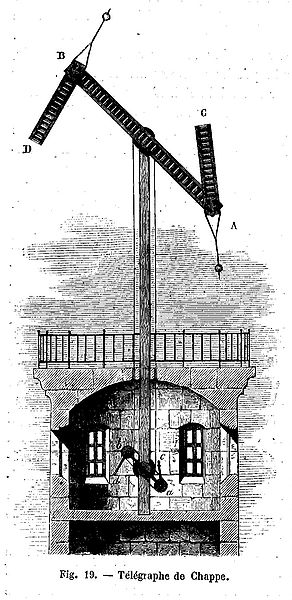
\includegraphics[width=0.3\linewidth]{chappe_tower}
\end{figure}

Similar to how we used human arms to communicate during our game of catch, the arms of the tower could be given many different positions, each corresponding to a different letter or phrase. The advantage of the mechanical arms over human ones, of course, is that the arms on the tower are much larger and hence can be seen from further away, stretching the distance between two towers.

Since this first telegraph was to be used for strictly military purposes, the meaning of the arm positions that emanated from the towers was to be kept secret. In fact, even the operators of towers often were simply mimicking the arm positions of the transmitting tower, without knowing the meaning of the message contained within that series of arm positions. [CITE]

The first line of these towers between Paris and the town of Lille was completed in 1792. Once this proof of concept was established, the telegraph network exploded and spanned much of France within half a decade, demonstrating the utility of telecommunications:

\begin{figure}[H]
\centering
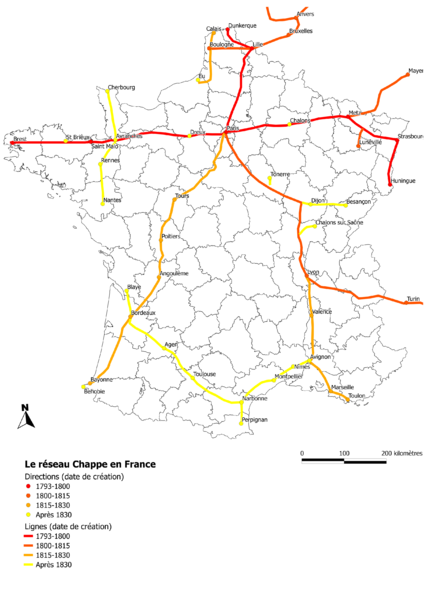
\includegraphics[width=0.5\linewidth]{chappe_network}
\end{figure}

This was the world's first extensive telecommunications network, and it required no wires at all.

The network in France was copied in other countries, as telegraph towers started appearing all over. In fact, if you live in a hilly city, you may have a neighborhood nearby called \emph{telegraph hill}; this name is derived from the hills upon which optical telegraphs were placed to maximize visibility.

\section{Efficient Communication}

We've seen how a semaphore system can be used to create a one-to-one correspondence between arm positions and letters of the alphabet. The system used by Chappe's towers was very similar to our example holding flags:

\begin{figure}[H]
\centering
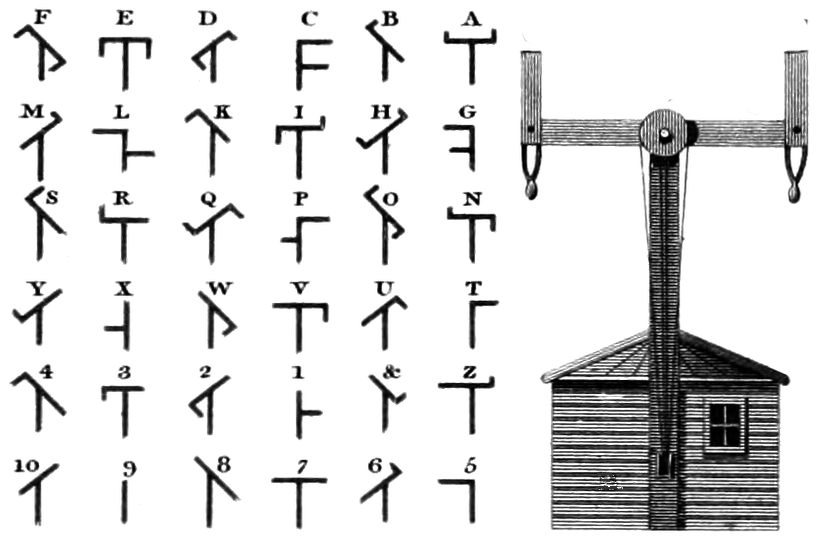
\includegraphics[width=0.5\linewidth]{chappe_telegraph_system}
\end{figure}

It is easy to imagine how this could be used to convey arbitrarily long text. However, while the system was general enough to allow for entire sentences, it was often not practical to send full sentences when less information was needed.

To understand why, consider that the time it takes to transmit a message grows with the number of letters, since, for each letter, an operator in a tower has to shift the mechanical arms of the tower to the position corresponding to that letter. As a back of the envelope calculation, let's estimate that it takes 30 seconds to change the position of the large mechanical arms to form a letter, and another 30 seconds of waiting to ensure the next relay station down the line got a good view of the letter. That means it takes 1 minute per letter, and so a sentence made up of 14 letters might take 14 minutes to go from one tower to the next. If there are 30 such towers each 10 miles apart, transmitting your 14-letter message across a distance of 300 miles will take 14 minutes $*$ 30 towers, or 7 hours. Still faster than horseback, but only slightly.

We can greatly improve the efficiency of the system if the tower operators simultaneously transmitted and received; in other words passing letters down the line one at a time. This helps, but also makes the system more prone to error, since it requires operators to synchronize their operating speed, else letters could get missed. Without getting too deep into the tradeoffs between speed and effectiveness in transmission, sending longer messages was clearly challenging. On the other hand, sending short messages was generally much easier. A message of a single letter, for example, could traverse the entire 300 mile semaphore line in $1 * 30$ = 30 minutes, an order of magnitude faster than a horse can ride. Given the advantages of short messages, it was almost certainly the main mode of communication in early optical telegraph systems. [TODO RESEARCH IF RECORDS EXIST]

For example, suppose a military commander in Paris knew that a certain foreign adversary might march their troops to the capitol, or might instead pull back. Let's suppose this was \emph{binary}: either troops are coming to the capitol or they aren't. To indicate this, a general on the front lines could send a full sentence, such as:

\begin{quotation}
Foreign troops are en route to Paris
\end{quotation}

But as we've seen, this would be overkill and unnecessarily taxing on the semaphore line. Instead, all the general needs to send is a yes-or-no, a single \emph{bit} of information. To accomplish this, it would suffice to send a single character encoded as a single arm position. Arbitrarily, let's say that the general agrees to send the arm position corresponding to 'B' if the troops are en route to Paris, and the arm position corresponding to 'A' if they have pulled back.

\begin{align*}
	A&: \text{enemy army pulled back} \\
	B&: \text{enemy army marching to Paris}
\end{align*}

How many possibilities can the general send with just a single letter? The set of arm positions forms an \emph{alphabet} with 36 characters, and so with one character there are 36 different possible messages that one can produce. You might imagine, for example, that the French army had 36 different important phrases that were understood to be encoded by single characters:

\begin{align*}
	A&: \text{enemy army pulled back} \\
	B&: \text{enemy army marching to Paris} \\
	C&: \text{need more food supplies} \\
        D&: \text{need more weapon supplies} \\
        E&: \text{we are defeated in battle} \\
        \text{etc} &
\end{align*}

What if the French army decided that 36 phrases weren't enough to capture all of the messages that they wanted to send? Of course they could always fall back on using the optical telegraph network to convey full sentences, but before doing that, it surely makes sense to create codes of 2 letters, e.g.

\begin{align*}
	AA&: \text{enemy army remains at camp} \\
	AB&: \text{enemy army deserting camp and returning to base} \\
	AC&: \text{enemy army splits; some at camp, some returning to base} \\
        \text{etc} &
\end{align*}

How many messages could be sent with two letters? Each of the two characters can range over 36 possible values, giving us $36*2=36^{2}=1296$ possible 2-character messages. Similarly, there are $36*36*36=36^{3}=46656$ three-letter configurations. And more generally, with $n$ characters, we number of possible messages that can be produced is $36^{n}$. This can get large quite quickly, demonstrating the power of exponential growth.

\begin{align*}
1 \text{ letter} &= 36 \text{ configurations} \\
2 \text{ letters} &= 36*36 = 36^{2} = 1296 \text{ configurations} \\
3 \text{ letters} &= 36*36*36 = 36^{3} = 46656 \text{ configurations} \\
4 \text{ letters} &= 36*36*36*36 = 36^{4} = 1679616 \text{ configurations} \\
5 \text{ letters} &= 36*36*36*36*36 = 36^{5} = 60466176 \text{ configurations} \\
6 \text{ letters} &= 36*36*36*36*36*36 = 36^{6} = 2176782336 \text{ configurations} \\
7 \text{ letters} &= 36*36*36*36*36*36*36 = 36^{7} = 78364164096 \text{ configurations} \\
&\text{etc}
\end{align*}

That's a lot of information that can be sent with 7 characters! As a point of comparison, there are only 51339 English words that are 7 letters or less, according to the pared down Scrabble dictionary.

\subsection{Entropy}

In order to capture the notion that the above system of codes is generally more efficient than natural language, it is prudent to introduce the idea of \emph{entropy}, which is a measure of unpredictability of information content. Messages that are highly structured and predictable have low entropy, whereas unpredictable sequences are densely information-packed and thus have high entropy. The concept of entropy was first introduced in the context of thermodynamics in the 19th century, as a measure of, roughly, the orderliness of a thermodynamic system. The word was then co-opted by the mathematician Claude Shannon in the 1940s (on the advice of another famous mathematician, John von Neumann) to the context of \emph{information theory}, and it is this information-theoretic sense of the word that is important for our purposes.

To get an intuition for entropy, let's consider a simple example. Suppose you are generating a very silly message by flipping a coin 10 times and recording the result after each flip as a $H$ or a $T$. In this example, each letter can be viewed as a \emph{random variable} that takes on one of two values. With a fair coin, you might end up with a message that looks something like: $HTTTHHTHTT$. This has high entropy since each coin flip gives you a lot of information about the sequence.

Now, consider another sequence generated by flipping coins and only writing down the value if it is heads, ignoring any tails flip. This will give you the same boring sequence in every scenario: $HHHHHHHHHH$. This has low entropy (in fact, zero) since it is incredibly predictable and structured.

Finally, consider a third example, in which you generate a sequence of 10 letters through the following procedure: flip a coin, and write the value down twice. Doing this five times gives you a sequence of ten letters that could look something like $TTTTHHTTHH$. In this case, letters in the sequence are alternatively random and completely redundant. As you might guess, this string has lower entropy than the completely randomly generated string, but higher entropy than the boring sequence of only heads.

Returning to the Chappe telegraph network, we can restate what we discussed above in terms of entropy by observing that natural languages like English (or French) have fairly low entropy. For example, suppose you are reading an English sentence one letter at a time. After the letters 'communica' appear, the next letter is virtually certain to be a 't,' which makes the letter extraneous much like our redundant coin flips above. As another motivating example of why English is low entropy, consider the fact that when writing English, you can skip or mistype letters a fair amount, and yet the meaning will still be clear to readers:

\begin{quotation}
\centering
\emph{Dos ths maake setnse?}
\end{quotation}

In contrast, the system of coded messages was designed with efficiency in mind, and each letter is of critical importance. The message 'a2r' and the message 'a2t' might signify completely different things, and so that typo could prove disastrous. This means the coded messages have a much higher entropy than English, without redundant information; this means that more can be communicated with fewer characters.

Despite the intuitive importance of creating communication systems that were more efficient than natural language, it would take over a century before the mathematics behind these ideas came sharply into focus thanks to the groundbreaking work of Claude Shannon. Fortunately, progress did not stall for lack of a mathematical theory of communication. As towers were being built in France to expand the telegraph network under Napoleon in the early 1800s, forward-thinking inventors were starting to see promise in developing a communication technology based on electricity.

\chapter{The Electrical Telegraph}

One major limitation of Chappe's telegraph network is that it relies on line of sight. What happens if it gets foggy? Or if you want to communicate across a large body of water that doesn't allow for the construction of towers along the way?

The electrical telegraph solves these problems, providing a more robust solution to long distance communication. As we will see, electricity traveling over a wire can be made into a fundamental building block for developing a system of communication. This approach doesn't have the shortcoming of the line-of-sight approaches – the wires can snake around large mountains, go through hazardous terrain, and lie at the bottom of large bodies of water. Moreover, electrical telegraphy doesn't require expensive towers to be built and maintained, and wires can fairly easily be re-positioned, making a network based on the electrical telegraph much less expensive and more flexible than one based on the optical telegraph paradigm.

Given all the advantages of the electrical telegraph, it is no surprise that shortly after being successfully prototyped in the 1840s, it eclipsed the optical telegraph as the dominant mechanism for communicating at a distance, and nowadays when someone talks about the ``telegraph'' they are almost certainly referring to the electrical telegraph. I will follow this convention, and explicitly use the phrase ``optical telegraph'' when I need to refer to the older line-of-sight-based Chappe technology.

The development of the electrical telegraph occurred in the first half of the 19th century, and relied on advances in battery technology and a steady progression in our ability to harness electricity in increasingly sophisticated ways. The telegraph served as society's first widespread proof in the power of electricity, and, much like the early 21st century, the mood was jubilant about what could be accomplished through further technological progress.

Like many great inventions, the ideas behind the telegraph were developed more or less independently by more than one person, and, like many great inventions of the modern legal era, bitter patent lawsuits were not far behind. The man who has ended up getting the majority of the credit as the father of the telegraph is Samuel Morse, an American painter-turned-inventor who was born in 1792, just as Chappe was furiously iterating on his towers half a world away. Morse was unaware of telegraphy of any sort through his early life. He painted portraits through his 30s and only in his 40s turned his attention towards electricity and the idea of creating a system of communication using electricity over a wire. He then obsessively worked on this problem, eventually developing and popularizing the dominant telegraphy system which became the standard used throughout the world for the next sixty years.

Besides Morse, the other prominent pair of inventors were Cooke and Wheatstone, who worked in England, independently developing their own systems for how to communicate over a wire. Conceptually, all of these people were on a similar track, but Morse's system had certain advantages over that of Cooke and Wheatstone, and eventually the world settled on the ``Morse system'' as the superior technology.

\section{A Simple Circuit}

The Morse telegraph is in essence just a simple electrical circuit. There is a power source, a switch and a loop of wire connected to an electrical device that acts as a receiver indicating whether or not electricity is flowing through the circuit:

\begin{figure}[H]
\centering
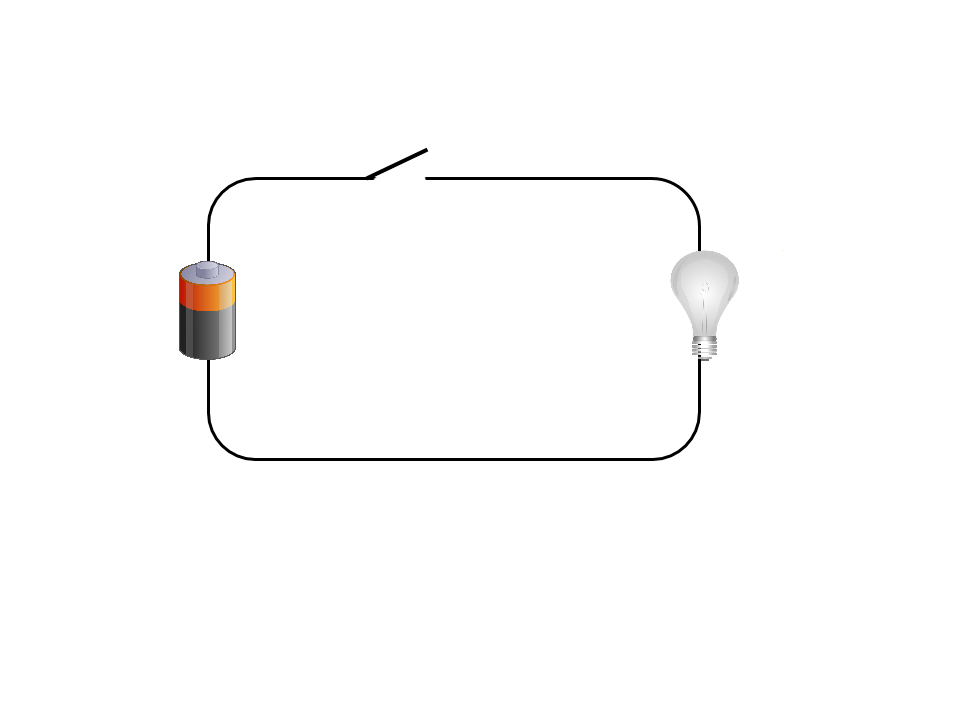
\includegraphics[width=0.8\linewidth]{circuit1}
\caption{Switch closed; no electrical current}
\end{figure}

In the circuit diagram above, the power source is the battery drawn on the left. The little angled line represents a \emph{switch}, and works just like a light switch in being able to turn the system on or off (in fact, light switches are essentially just switches in the sense of a simple circuit). If the switch is open, as it is in the diagram above, electricity does not flow through the circuit. If the switch it closed, on the other hand, then an electric current flows from the negative end of the battery through the circuit to the positive end of the battery:

\begin{figure}[H]
\centering
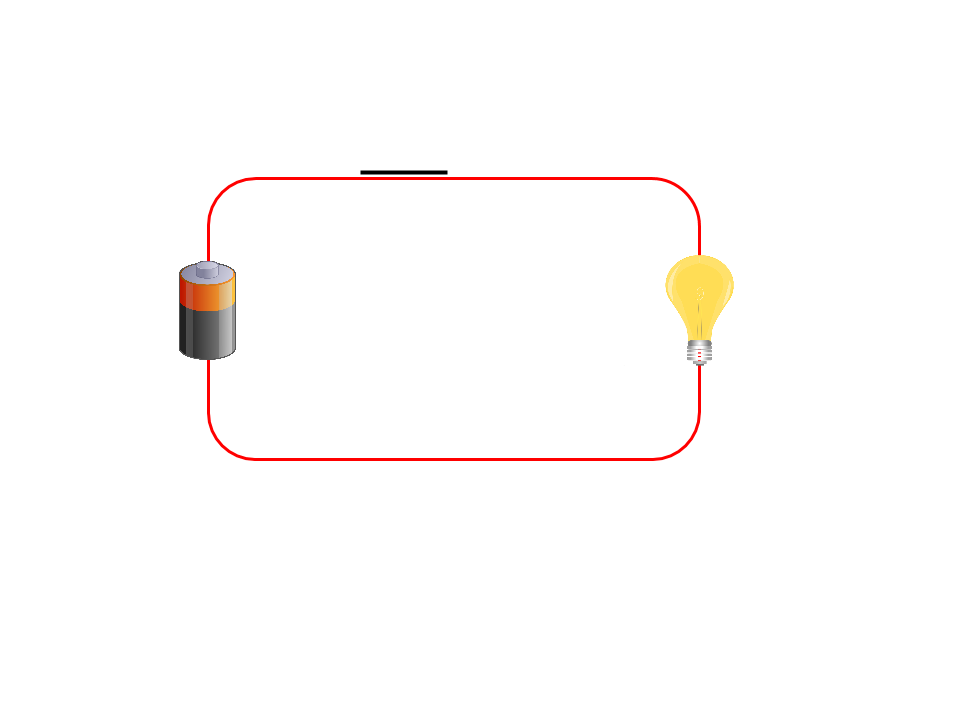
\includegraphics[width=0.8\linewidth]{circuit2}
\caption{Switch open; electricity flowing}
\end{figure}

Typically in elementary electrical engineering explanations, a light bulb is used as an illustration of this electrical device indicating that electricity is flowing through a circuit, and so we have used this above as a simple illustration. Unfortunately for Morse and his peers, there were no light bulbs in the 1830s and 1840s, but there were alternatives serving the same conceptual function as a light bulb in the diagram above.

\section{One Telegraph to Rule Them All}

While all electrical telegraphy developed through the 1840s was based on the paradigm of a simple circuit that we described above, the details varied quite a bit among competing designs. There was not a single telegraph during this period, but rather a plethora of distinct competing experimental systems for communicating over electrical wires.

Early designs often involved creating many circuits, even one per letter of the alphabet. To take one prominent example of a many-circuit design, in England in the late 1830s, Cooke and Wheatstone developed a working prototype of a telegraph that involved six wires. On the receiving end of this telegraph, there were five needles that could be made point to a particular letter. The receiver looked something like this:

\begin{figure}[H]
\centering
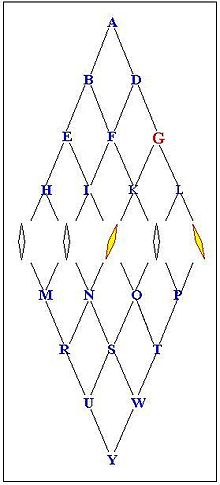
\includegraphics[width=0.4\linewidth]{wheatstone}
\caption{Cooke and Wheatstone telegraph receiver. Notice the two non-vertical needles pointing at 'G'.}
\end{figure}

The transmitting signals would affect the position of the needles via magnetism, and by altering two needles at a time, the transmitter could use the two needles to point at a letter of the alphabet on the receiver board. One interesting feature of the Cooke and Wheatstone telegraph that you may have noticed is that it does not provide a complete alphabet: J, Q, and Z are missing. This was unfortunate but not devastating, since, as we've seen, the entropy of natural languages like English are rather low and so one can still get meaning across with quirky spellings.

When the dust settled, however, the telegraph that became the de facto worldwide standard was a design coming from Morse and his collaborators, notably Alfred Vail. As we will see time and time again, simplicity is a major virtue when designing a telecommunications system, and by requiring only a single circuit for transmission, Morse's telegraph system had a major advantage over other early prototypes.

Let's look in a bit more detail at how the Morse telegraph worked. Here is a representation superimposed on our basic circuit above:

\begin{figure}[H]
\centering
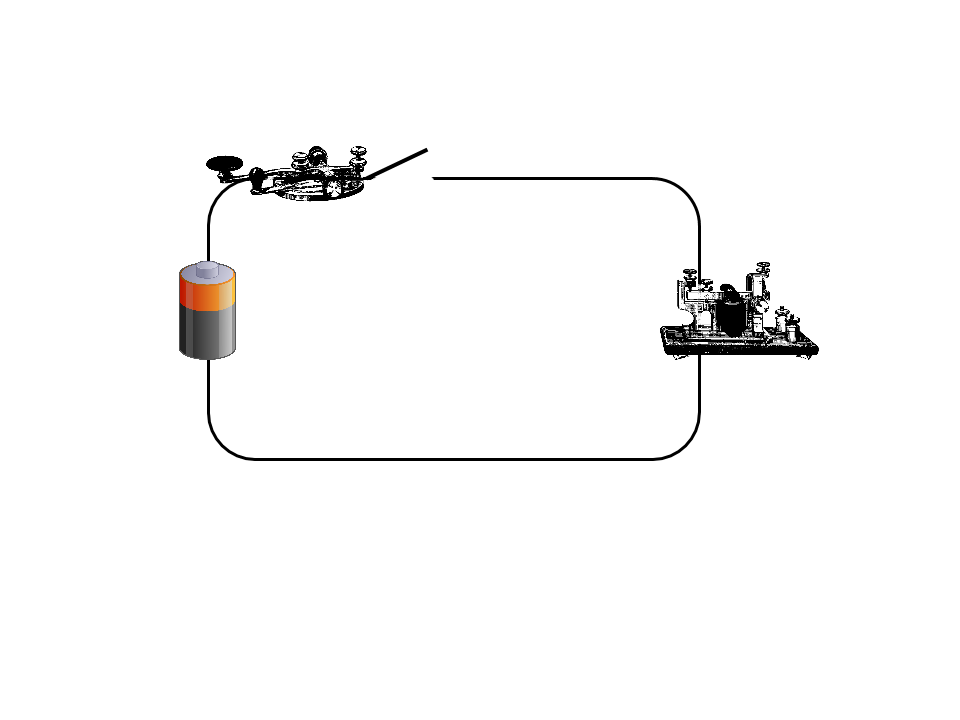
\includegraphics[width=0.8\linewidth]{telegraph_as_circuit}
\caption{Telegraph as a basic circuit}
\end{figure}

The circuit was closed by default, which means that electricity was flowing through. Transmission occurred via a \emph{telegraph key}, an invention of Vail that was essentially a single button that an operator could press. When pressed, the circuit was opened and electricity no longer could flow through the wire. When released, the circuit was closed and electricity resumed.

\begin{figure}[H]
\centering
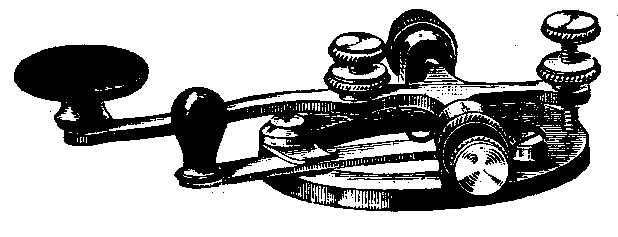
\includegraphics[width=0.6\linewidth]{telegraphkey}
\caption{Telegraph key}
\end{figure}

Telegraph operators would tap out messages with this single key in a specified manner (which we'll discuss shortly).

There was a bit more variance over the life of the telegraph in terms of what gadget was actually used to \emph{receive} messages. After experimentation with all sorts of receiving devices –- making little marks on paper, making needles point to particular locations, and so on -- the winning gadget employed throughout the peak of the telegraph in the mid to late 1800s was called a \emph{sounder}:

\begin{figure}[H]
\centering
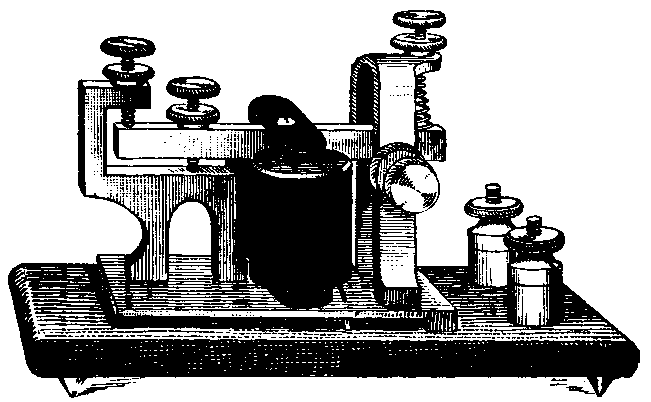
\includegraphics[width=0.6\linewidth]{telegraphsounder}
\caption{Sounder}
\end{figure}


This device allowed telegraph operators to listen to clicks and pauses which corresponded to the pressing and lifting of the telegraph key by the operator at the other end of the line.

We now have a clearer picture of the mechanics of how a telegraph worked: it was essentially a circuit with a key on one end corresponding to a switch and a sounder on the other end that allowed key presses to be heard as clicks.

\section{Morse Code}

Knowing that someone on the other end of a telegraph line hundreds or thousands of miles away is pressing a key at this very moment is a remarkable achievement, but in order for it to be useful for communication, there needs to exist some \emph{system} that translates the ``on'' and ``off'' states of the telegraph into useful information.

We've discussed a couple such systems for communication already, but these relied on line of sight and being able to display lots of information at once, either in the form of varying arm positions or in various lights that are on or off. In this case, we only have a single on or off state that can change over time. How can this be used to convey information?

The system that stuck for telegraphy is known as Morse code. Morse code enables communication by segmenting the raw ``on'' and ``off'' states into four discrete symbols: a dot, a dash, a short pause, and a long pause. A short press of the telegraph key was called a ``dot'' and a long press of the key was called a ``dash''. Different lengths of pauses were necessary to differentiate a pause between letters from a pause between words.

\begin{center}
\begin{tabular}{cc}
\thickdot & dot \\
\hline
\thickdash & dash \\
\hline
[short pause] & letter space \\
\hline
[long pause] & word space \\
\end{tabular}
\end{center}

These four symbols comprise the basic alphabet of telegraphy, but we also need a way to translate this basic alphabet into English letters, much as we did for our system of lights earlier. It is not too difficult to create such a table:

\begin{figure}[H]
\centering
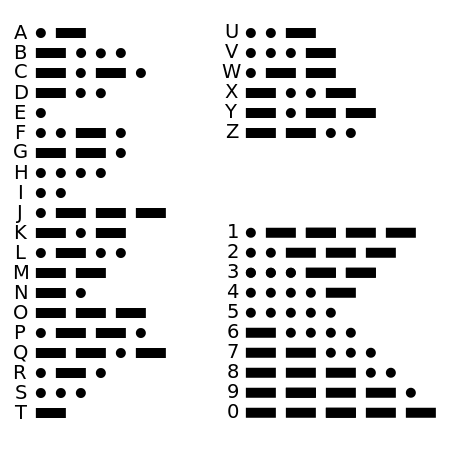
\includegraphics[width=0.8\linewidth]{morse-code}
\caption{International Morse Code standard}
\end{figure}

Armed with this system, the telegraph is transformed from a meaningless single-signal transmission device into the world's first widespread telecommunication technology. The way it works is similar to the semaphore system we outlined above. For example, consider the following sets of dots, dashes, short pauses and long pauses, represented on paper via our table above:

\[ \thickdot \thickdot \thickdot \thickdot \quad \thickdot \quad \thickdot \thickdash \thickdot \thickdot \quad \thickdot \thickdash \thickdot \thickdot \quad \thickdash \thickdash \thickdash \]

Using the translation table, to which English word does this correspond?

As mentioned, the Morse system has the advantage that only a single circuit is needed to communicate, meaning that even very simple designs for the physical telegraph could be made to communicate via Morse code. In particular, unlike the more complex designs of Cooke and Wheatstone (as well as Morse's earlier systems), the telegraph which became the standard did not require multiple circuits to be synchronized with one another to produce an output, significantly cutting down the complexity of the system.

\section{Practical Limits of Telegraphy}

Despite a lack of theoretical understanding of the fundamental principles that enabled electrical telegraphy to function, early electrical engineers forged ahead in improving the telegraph. It didn't work perfectly, though, and so a lot of energy was spend trying to get telegraphs to be more reliable, to function over long distances, and to be able to cross harsh terrain.

One challenge at first seemed insurmountable: could a telegraph cable be built that traversed the Atlantic ocean?

To achieve this, improvements to cabling were critical. In particular, early telegraph systems involved stringing raw copper wire along poles, or burying it underground. But raw copper wire was unreliable as a transport mechanism: it could be easily damaged, and simply did not work that consistently even if undamaged.

For telegraphs to function at scale, more sophisticated cabling was needed. Fortunately, \emph{gutta-percha} was discovered by the industrial world in 1843 and quickly became a household name in the Victorian world. This tree sap known for producing a naturally rigid latex became the mid to late 19th century's equivalent of plastic today, and among its myriad uses was as an insulator surrounding raw copper telegraph wires. The gutta-percha in turn was often wrapped in rubber, and then an outer layer or iron or steel, creating a cable whose cross section looked something like this:

\begin{figure}[H]
\centering
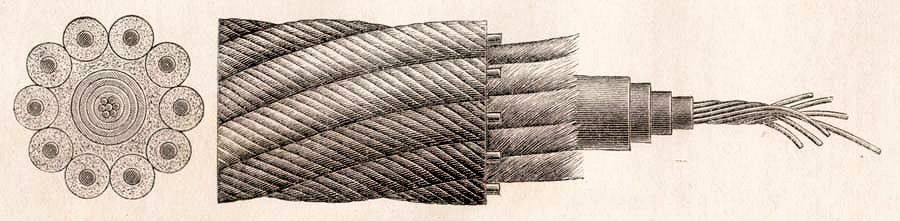
\includegraphics[width=0.8\linewidth]{cable-cross-section}
\caption{Telegraph cable}
\end{figure}

It did not happen overnight, but 14 years after Morse's first successful proof of concept of the electrical telegraph in 1844 between Baltimore and Washington, D.C., the first transatlantic telegraph cable was laid, ushering in the dawn of a new information age of instantaneous cross-continent communication. Imagine the jubilation one must have felt being in New York City in 1858, hearing Queen Victoria's words to president Buchanan that for the first time could be communicated near-instantaneously across the vast Atlantic ocean.

Meanwhile, engineers remained hard at work making improvements. In addition to better cabling, there were a lot of open questions. How thick should the copper wire be? How powerful should the battery be? The engineers involved in these early projects engaged in a tremendous amount of trial and error, and succeeded in pushing the range and reliability of telegraph lines despite limited theoretical understanding of electricity and magnetism.

Yet even as engineers inched towards cables that were better optimized for the task at hand, there remained one unfortunate fact of life: over longer and longer distances, the strength of the signal diminished.

This phenomenon, which in contemporary parlance is called \emph{attenuation} of the electrical signal, is due to the fact that energy escapes when electricity travels over a wire, diminishing the signal. (Energy escapes as heat, for example, making wires warm and turning them into an attractive hang out location for birds). To solve the fact that the signal would get weaker over longer distances, some sort of repeating mechanism was needed. One could set up telegraph stations with human operators every so often to serve as this repeating mechanism, much like the relay towers of the optical telegraph, but that would be expensive and unfeasible in some cases depending on the terrain. Fortunately, there was a way that signals could be repeated without the need for intermediate stations operated by humans.

\section{Electromagnets and Relays}

In order to understand the repeating mechanism that became standard, we must first understand an electrical device invented in the 1820s called an \emph{electromagnet} which serves as a basic building block for many electrical systems.

You can think of a simple electromagnet as a piece of iron with insulated wire tightly coiled around it:

\begin{figure}[H]
\centering
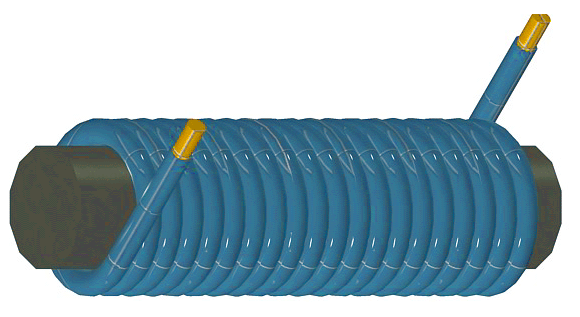
\includegraphics[width=0.8\linewidth]{electromagnet}
\caption{Simple electromagnet}
\end{figure}

When current flows through the wire, it induces a magnetic field, turning the iron temporarily into a magnet that attracts other metals. In other words, with an electromagnet, the flow of electricity is used to dictate whether a magnet is ``on'' or ``off''.

One of the reasons the electromagnet is so important is that it allows electrical current to create mechanical action. To see how this is possible, consider the following setup:

\begin{figure}[H]
\centering
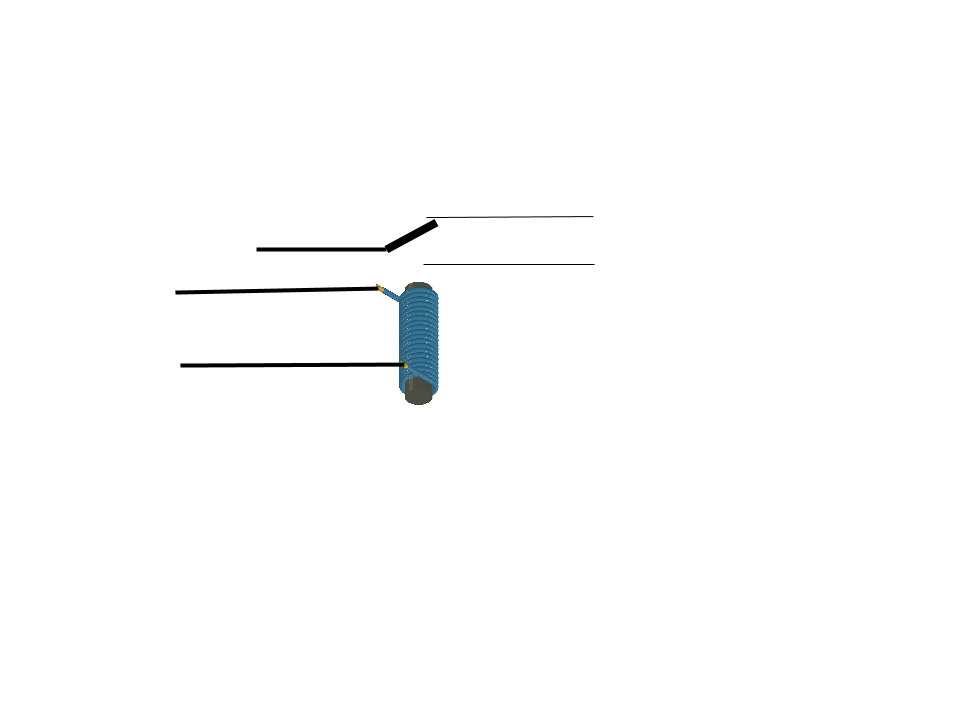
\includegraphics[width=0.8\linewidth]{electromagnet_with_latch}
\end{figure}

When electricity flows, the electromagnet is activated, creating a magnetic field, which pulls the metal latch down.

\begin{figure}[H]
\centering
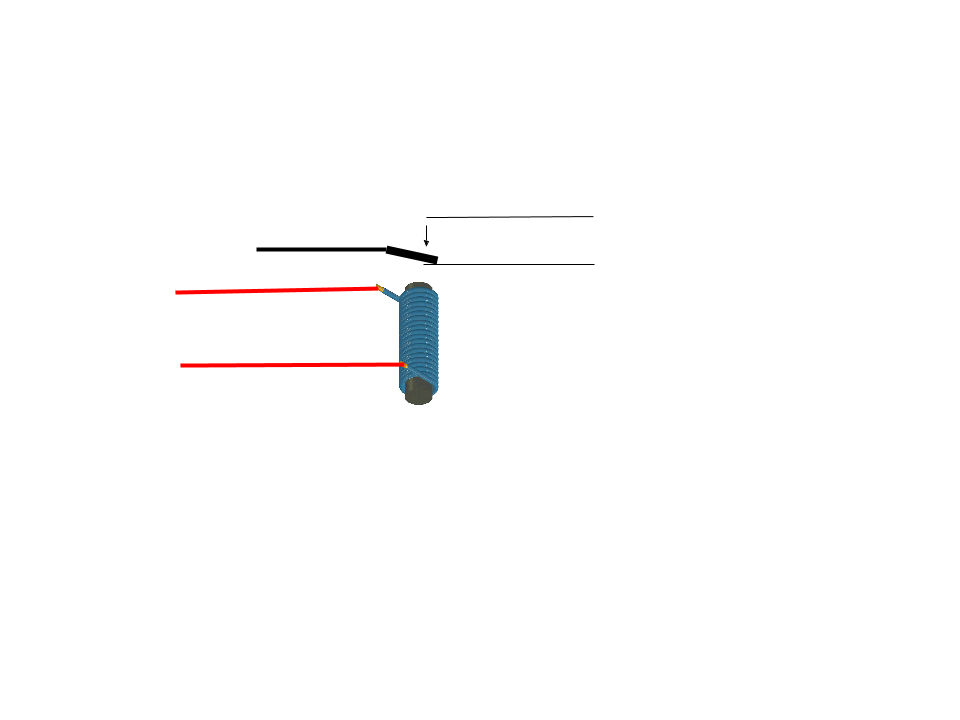
\includegraphics[width=0.8\linewidth]{electromagnet_with_latch_2}
\end{figure}

When the flow of electricity stops, the magnetic field disappears and the latch returns to its original position. Now what if the metal latch that is going up and down is actually the switch of another electrical circuit? You can now have two circuits with independent power sources linked by this electromagnet like this:

\[ [DIAGRAM] \]

An electromagnet used in this way is called a \emph{relay}. Imagine the left side of the above diagram as a telegraph operator using a telegraph key. When the operator presses down, communicating a dot in Morse code, it opens the switch and cuts the electrical current for a brief moment. This causes the magnetic field to disappear in the electromagnet, and so the latch in the relay returns to its original position, which breaks the current on the right hand side, communicating a dot.

By offering a way around the signal attenuation issue, relays allowed telegraph lines to extend arbitrarily far. Of course relays were yet another piece of equipment that had to be installed and maintained, but this was far less costly and more flexible than having many staffed telegraph offices responsible only for repeating a signal.

Electromagnets had another important purpose. Recall that a sounder was used at the receiving end of telegraphs to listen to the dots and dashes of Morse code. But how did a sounder actually work? It was in fact an electromagnet that worked just like a relay, except that instead of controlling another circuit, the latch going up and down made respective and distinct ``click'' and ``clack'' sounds, allowing operators to identify difference cadences of clicks and clacks with the Morse code alphabet, which they could in turn decode into English.

\chapter{Symbolic Systems}

Having taken the time to learn about early telegraphy systems, let's step back and discuss some important elements of communications systems more abstractly. First, we can introduce the dominant paradigm for conceptualizing a communication channel:

\begin{figure}[H]
\centering
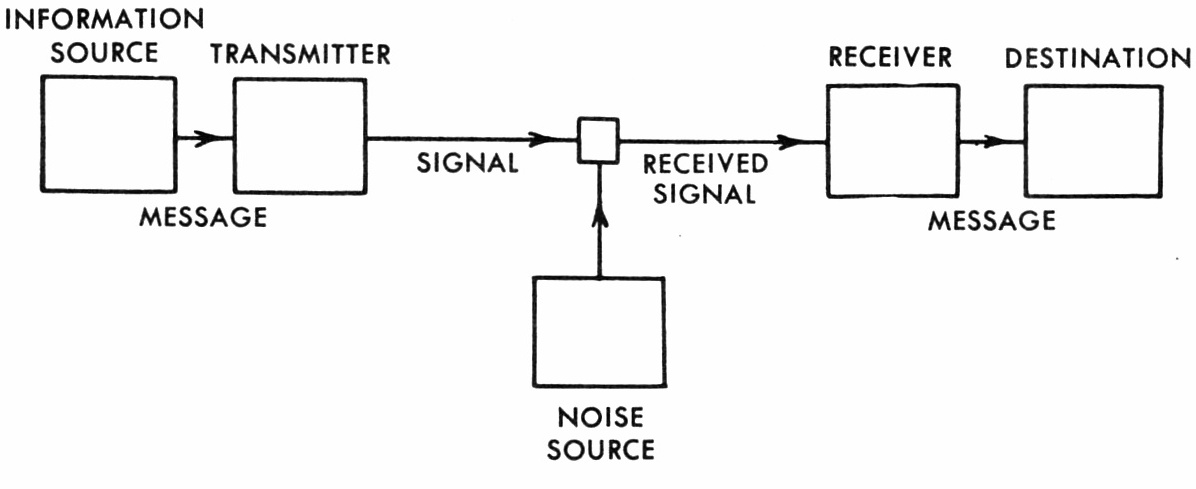
\includegraphics[width=0.8\linewidth]{shannon_comm_channel}
\caption{Shannon's Fundamental Model: an abstract representation of a communication channel}
\end{figure}

This image is taken directly from a 1948 paper by the mathematician Claude Shannon, and is still the same model in use today, demonstrating Shannon's incisive ability to give very clear and compelling guide posts for how to think about information and communication. Let's call this \emph{Shannon's Fundamental Model}. Shannon created this diagram in an era where telephones and radios were prominent, but it nevertheless pertains to the telegraph as well, a fact noted by Shannon in his paper. In the above image, the box in the middle represents the information \emph{channel}. Depending on context, this could be the air between two optical telegraph towers, a telegraph wire, or something else. The signal being transmitted is the message, and the noise source represents the ways in which the message might get scrambled in the channel. The word \emph{noise} appears for historical reasons: anyone listening to a telegraph or telephone line would hear a lot of hissing, crackling, or buzzing sounds and this was a nuisance for communicating; \emph{noise}, then, became the abstract word to refer to any exogenous factor that might add difficulty to communicating. For example, on a foggy day, it may be difficult to see an optical telegraph tower and so as an operator you might be more inclined to make a mistake about the arm positions of an adjacent tower. In this scenario, we might say that the fog is the noise source, and the less transparent air is the resulting noise. The transmitter and receiver are represented in order to suggest that ordinarily messages have to be encoded before they enter the communication channel, and then decoded once the received signal has reached its destination. We've seen this already, for example, with both the optical and the electrical telegraph. For the latter technology, messages have to be translated into dots and dashes, and then to electrical signals, which get communicated via the telegraph wire before being decoded back into dots and dashes and ultimately into a message of letters.

Beyond Shannon's Fundamental Model, there is an incredibly important distinction between two classes of communication systems. All of the communication systems we've discussed so far have been \emph{symbolic} in nature, involving the transmission of a number of symbols. But there is another type of communication entirely different from conveying symbols. Consider the human voice. The pitch rises and falls along a spectrum. There aren't only $5$ or $50$ or even $5000$ possible values for the pitch of the human voice. Instead, the pitch can vary infinitely, and this makes pitch of the human voice a \emph{continuous} variable, in contrast to the \emph{discrete} variables that only take on one of some fixed finite number of values (for example, letters in the alphabet).

Another example of a continuous variable is human height. Adult humans tend to be between 1 and 9 feet tall, but adult human height is nevertheless a continuous variable, meaning that like the pitch of your voice, there is no finitely enumerable set of possible height values. Instead, there are an infinite number of values between 1 and 9 feet that could represent human height. Communication systems that are able to communicate continuous variables are called \emph{analog} and we will get a much closer look at some of these in the next chapter. In contrast, communication systems that are based on a fixed and non-infinite set of symbols are called \emph{symbolic} communication systems.

Unlike the telephone, broadcast radio and television technologies that succeeded it, which were all based on the analog paradigm, the telegraph is a symbolic communication system just like the Internet. That makes it particularly suitable for introducing important concepts related to symbolic communication and how the Internet is structured.

\section{Alphabets and Symbols}

Consider the letter \emph{`a'}, the first letter of the Latin alphabet. What makes this mark meaningful? If we did not know English or any other languages based on the Latin alphabet, then \emph{a} would just appear to be a mysterious mark with no meaning, such as $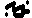
\includegraphics{randomsymbol}$.

Thus for the letter \emph{a} to carry information for the onlooker, it has to exist within the context of an \emph{alphabet}. Let us call `a' a \emph{symbol} or \emph{character}. Note that `a' has abstract meaning: we could write it in a different font like this: {\fontfamily{qcr}\selectfont a}. But even though the marks appear differently when represented in different fonts, the mark has enough structural similarity that we recognize both marks to refer to the same abstract character `a.' Of course the Latin alphabet is not the only meaningful alphabet; the Chinese character 章 may look meaningless to a non-Chinese reader, but it certainly has meaning within the context of the Chinese alphabet.

What about a number like \emph{2}? You might be inclined to think that this is not part of an alphabet, since it is a number and not a letter. However, for our purposes, we are intentionally going to use the word \emph{alphabet} very broadly, as logicians do, as a fixed set of symbols that are distinguished from one another by some known rules or conventions. Note that this broad definition does not say anything at all about what the symbols \emph{mean}, and so any sets of symbols that go together can be said to form an alphabet. In particular, the symbols $0, 1, 2, 3, 4, 5, 6, 7, 8, 9$ do indeed form an alphabet that usually goes by the name \emph{the Arabic numerals}.

We will refer to a series of characters of an alphabet as a \emph{string}. So, for example `119914' is a string in the alphabet of Arabic numerals, and `sdklfsid asdfasdf' is a string in the alphabet of Latin characters. Strings are always relative to some alphabet.

There are some interesting edge cases. What about alphabets that contain infinitely many symbols? Or symbols that are fuzzy and so it is not always possible to tell two symbols in the alphabet apart? With a bit of mathematical formalism, we could sharpen the discussion of these edge cases, and join a community of logicians who actively discuss these topics. [CITE ENDERTON]. Fortunately, for our purposes we can dismiss these edge cases and insist that the symbols are all easily distinguishable from one another and that there are only a finite number of these symbols.

That's enough background to establish our first major proposition about symbolic systems.

\begin{theorem}
Suppose $s$ is a string of some alphabet $A$. Then for any other alphabet $B$ that has at least two symbols, $s$ can be represented in $B$ via a new string $s'$ without any loss of information.
\end{theorem}

This is a slightly formal way of saying that all symbolic representations are interchangeable. If you have some string in one language, like the string ``hello'' in the alphabet of Latin characters, then by fixing some translation system, one can represent this as a number (i.e. a string in the alphabet of Arabic numerals). To unpack this a bit more, let's consider an example sentence:

\begin{quotation}
\centering
\emph{All symbolic representations of information are fungible!}
\end{quotation}

How could we represent this string via another alphabet? For starters, we could translate this to the Chinese alphabet, giving us a new representation of the sentence:

\begin{quotation}
\centering
\emph{所有的信息符號表示是可替代的!}
\end{quotation}

I mentioned above that one had to agree on a translation system.  Which one was employed for this translation? We might call it a \emph{semantic} translation system in that the underlying meaning of the sentence was recreated via a new sentence in Chinese. This is actually a tremendously difficult, imperfect and complicated translation system, as evidenced by the fact that non-human translations still lag far behind human translators as of 2015. Fortunately, we can also come up with much simpler translation systems.

To see this, let's translate the above sentence into Arabic numerals. \emph{Guh? How can you translate a sentence into numbers!?} The important thing to remember is that we get to decide on the translation system. In this case, we can pick something arbitrarily, just like we did earlier during our game of catch with Mary. Let's just translate each letter to its position in the alphabet:

\begin{quotation}
\centering
\emph{1 12 12  19 25 13 2 15 12 9 3  18 5 16 18 5 19 5 14 20 1 20 9 15 14 19  15 6  9 14 6 15 18 13 1 20 9 15 14  1 18 5  6 21 14 7 9 2 12 5 !}
\end{quotation}

This \emph{almost} counts as a translation into the 10-symbol Arabic alphabet that we specified above. But there is a subtle issue that we need to deal with: we still have the whitespace character ' ' and the `!' character, neither of which occur in the Arabic alphabet. You might counter that neither of these are considered part of the 26-character Latin alphabet that underlies English. But remember that we are using the word alphabet in a particular sense, and in this more formal sense, any alphabet that underlies ordinary written English must have symbols corresponding to whitespace, exclamation points and other pieces of punctuation, since these are part of the language. Put another way, if we formalize the written English language as a system for communication, it will necessarily include extra conventions beyond the Latin letters one learns in elementary school: to separate words, to separate sentences, to indicate questions, etc. The rules are easier to enumerate if we think about punctuation characters and whitespace characters as part of alphabet that makes up the language.

Therefore, to make our mapping to the alphabet of Arabic numerals a proper translation, we need a way to separate the words without using the space or exclamation point characters, neither of which we are available to us in our new alphabet. This isn't as trivial as simply removing the characters, since we need to away to disambiguate strings like '15' which could correspond either to `af' or `p'.

We also need this character separator to be some sort of number, in other words a string of one or more digits from 0 to 9. We didn't use the symbol `0' for any English letter, and it is available to us, so how about that? That almost works, except that there are still some ambiguous strings. For example, `2002' could translate into `b  b' or `t b'. We're getting closer, though. The problem with our current attempt at a solution is that each English letter could correspond to a variable number of digits. What if instead we enforce that every letter is exactly two digits long, so the letter 'a' is actually '01'? Now we can make '00' a space, and '27' an exclamation point. Moreover, we can also encode upper case letters and other common symbols as a sequence of two digits. Here is the whole table of our new translation system:

\begin{center}
\begin{tabular}{ cccccccc }
 00 & [space] & & 12 & l & & 24 & x \\
 01 & a & & 13 & m & & 25 & y \\
 02 & b & & 14 & n & & 26 & z \\
 03 & c & & 15 & o & & 27 & ! \\
 04 & d & & 16 & p & & 28 & ? \\
 05 & e & & 17 & q & & 29 & . \\
 06 & f & & 18 & r & & 30 & ' \\
 07 & g & & 19 & s & & 31 & , \\
 08 & h & & 20 & t & & 32 & - \\
 09 & i & & 21 & u & & 33 & / \\
 10 & j & & 22 & v & & \\
 11 & k & & 23 & w & & \\
\end{tabular}
\end{center}

Now we can successfully write the above sentence as a rather long number:

\begin{quotation}
\centering
\longnumber{4in}{01121200192513021512090300180516180519051420012009151419001506000914061518130120915140001180500062114070902120527}
\end{quotation}

With this, we have translated our sentence from the English alphabet into the alphabet of Arabic numerals. The giant number represented by the Arabic numerals has no inherent meaning, except when coupled with the translation system that we imposed earlier.

Let's compare this \emph{dumb translation} to the earlier \emph{semantic translation} into Chinese.

Given the semantic translation, a reader who did not understand English could understand the new Chinese sentence; given the dumb translation, on the other hand, there is no hope for this Chinese-speaker. The translated sentence still requires knowledge of English to be understood, and so in this sense the dumb translation is semantically vacuous.

Moreover, though it is vacuous, the dumb translation is also in some sense a perfect translation. Natural languages like English and Chinese are complex and messy tools for communication, and there is no way that the Chinese sentence created via the semantic translation perfectly captures the connotations wrapped up with the original English sentence. In that sense, information was lost translating to Chinese via the semantic translation. The dumb translation, on the other hand, merely involved manipulating symbols without any attempt at understand their meaning. Since it faithfully represented each and every symbol of the original English sentence perfectly, no loss of information occurred.

There is another word for performing a dumb translation like we did above: \emph{encoding}. The amazing thing about symbols is that they can be encoded without any loss of information, and you can encode any string of symbols into any other alphabet. The opposite of encoding is \emph{decoding} and refers to the process of backing out the original meaning from an encoded string.

Let's once again translate our original sentence into Chinese but this time with encoding rather than semantic translation. The Chinese alphabet has many more characters than the Latin alphabet, so we can pick 26 of these at random and create a translation table:

\begin{center}
\begin{tabular}{ cccccccc }
 吧 & a & & 爸 & l & & 八 & w \\
 京 & b & & 姐 & m & & 叫 & x \\
 很 & c & & 见 & n & & 家 & y \\
 会 & d & & 好 & o & & 海 & z \\
 百 & e & & 贵 & p & & \\
 过 & f & & 港 & q & & \\
 国 & g & & 儿 & r & & \\
 多 & h & & 东 & s & & \\
 关 & i & & 个 & t & & \\
 方 & j & & 哥 & u & & \\
 都 & k & & 对 & v & & \\
\end{tabular}
\end{center}

Luckily the Chinese alphabet also includes whitespace characters, so we do not need to do any extra work for this. Using this encoding, we get the following sentence, written with Chinese characters:

\begin{quotation}
\centering
\emph{吧爸爸 东家姐京好爸关很 儿百贵儿百东百见个吧个关好见东 好过 关见过好儿姐吧个关好见 吧儿百 过哥见国关京爸百!}
\end{quotation}

This will look like gibberish to a Chinese reader. Nevertheless, it is a faithful encoding of our English sentence, and armed with the encoding table above and knowledge of the English language, one can understand what it means.

Before moving on, let's ask one last question about encoding. As we've seen, you can encode any string of symbols into any other string in a different alphabet. Does this imply that there might be some \emph{best} way to encode information? The answer is that it depends on what you are trying to optimize. If you want to pack in as much information as possible into a small number of symbols (for example, if you are restricted to a single page of text), you might want to use a gigantic alphabet. For example, the Chinese alphabet has several thousand characters and would probably make a good choice.

It turns out, however, that the opposite optimization is actually much more important in practice. What is the \emph{minimum} bare bones alphabet that contains the smallest number of characters that we can use to encode information from other alphabets?

You might be tempted to say that you could create an alphabet of just a single character -- let's arbitrarily say `1' is the single character in this alphabet. Then you could distinguish strings by, say, line breaks:

\begin{quotation}
\centering

11111111 \\

vs \\

1111 \\
11111

\end{quotation}

Remember, though, that line breaks are themselves a character. So if you truly restrict yourself to a single character, there is no way to convey any information within a string other than the length of the string, which is too impoverished to allow for encoding. If you are unconvinced, try to encode the strings `hello' and `goodbye' in an alphabet of just a single character. If you think you have a translation system that works, continue adding words to it that you system did not anticipate having to be able to translate.

Though a one-character alphabet is not powerful enough to serve as a fully flexible translation system, what about a two-character alphabet? Let's call this alphabet \emph{binary} and name its characters `0' and `1'. With binary, we can faithfully encode information from any other alphabet with no loss of information. As an illustration, here is part of the American Standard Code for International Interchange (ASCII), a standard that we will meet later on that provides a way to encode Latin letters into binary (among other things):

\begin{figure}[H]
\centering
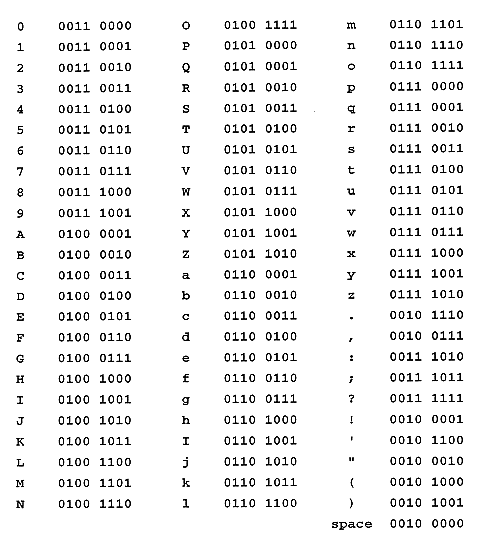
\includegraphics[width=0.8\linewidth]{ascii-binary-chart}
\caption{ASCII}
\end{figure}

Binary numbers are remarkable because you can add, subtract, multiply and divide them just as you can with decimal numbers.

IAMHERE

because you can compute with binary numbers just as you can with decimal numbers. You can add, subtract, multiply and divide binary numbers, and these operations on binary numbers are at the core of how computers work.

Much of the importance of binary stems from its importance to computing.

Given its simplicity and importance for computing, binary has become a sort of universal standard for understanding and communicating information.

\section{A Neatly Layered and Standardized System}

Although the idea of encoding information into a binary alphabet is incredibly well understood nowadays, this way of thinking about information and encoding and decoding was not around when Morse code was developed. Yet remember that Morse code has its own pared down four-character alphabet:

\begin{center}
\begin{tabular}{cc}
\thickdot & dot \\
\hline
\thickdash & dash \\
\hline
[short pause] & letter space \\
\hline
[long pause] & word space \\
\end{tabular}
\end{center}

This alphabet serves as an intermediary. It can be translated to and from electrical signals. It can also be translated to and from English. Since it operates by transmitting symbols back and forth, the telegraph is a symbolic communication technology. Moreover, since as we've seen all symbolic representations are interchangeable, any symbolic representation of information can be considered a representation in digits. Thus communication technologies based around conveying symbols are referred to as \emph{digital} and so we can say that the telegraph was a digital communication technology.

And as a digital or technology, the telegraph had to wrestle with many of the same questions that the Internet still wrestles with: how is digital information to be encoded and decoded? How will the process be standardized? Who will control the standardization process?

To begin to think about how to address these tough questions of how all the parts of the system would work together, the telegraph in contemporary parlance can be conceived of as a \emph{layered communication system}.

It's easiest to understand this through an example. Suppose you are sending a message to your friend Bill via telegram. Let's call the message `M'. We could also describe the communication as a series of letters being sent via telegraph. But we could also describe it at a lower \emph{layer} as a series of dots and dashes being transmitted back and forth. We can go to an even lower layer and find yet another description: electrical currents are turning on and off in rapid succession.

Let's zoom in on this example communication. A particular electrical current turning off might represent a dot, which might be part of the letter 'g' in your message. We could write this pausing of electrical current a few different ways:

\begin{quotation}
\centering
An electrical current is turned off and then on.
A dot is being sent.
A `g' is being sent.
The message `M' is being sent.
\end{quotation}

All of these descriptions are correct, but they are describing what is happening at different layers of the communication system. In the case of the telegraph, we can represent our layered system like this:

[DIAGRAM :
A. The physical layer of the electrical signal sent over the wire.

B. The translation of “signal on” and “signal off” into a very simple alphabet of dots, dashes, and spaces.

C. A translation of the simple alphabet of dots and dashes into the 26-letter alphabet (or more if we include extra characters such as spaces and special characters '?') of the English language.

D. A set of standards and abbreviations that telegraph operators used to communicate. For example, there is a standard shortcut for asking someone to retransmit a message [WRITE MORE ABOUT ITU?]
]

Thinking about communication technology as a layered system in this way allows us to break down the system into component parts, and has the huge advantage that layers of the system can now be changed without changing everything all at once. For example, suppose there was an improvement to Morse code that was proven to be a more efficient translation of dots and dashes into the Latin alphabet. Then layer C above could be changed, but nothing else would have to change; you wouldn't need to invent new electrical gizmos to transmit or receive messages. Conversely, suppose the technology for the physical layer vastly improved and electricity were replaced with a more advanced technology like optical fibers, as would happen a hundred years later. In this case, we could still use Morse code if we wanted, and so layers B-D would be unperturbed by changes in layer A. This makes the whole technology more manageable, since some engineers can go off and work on improving layer A and others can work on improving layer B and they do not both need to holistically invent a whole new communication system.

The Internet is also built upon a layered system of communication, which we'll learn about later on.

\subsection{Metadata}

We've discussed layers A, B, and C in some detail already, but it's worth pausing to think about what layer D above might look like.

To emphasize the importance of layer D, suppose you are a telegraph operator sitting in a local telegraph station in Idaho in the 1880s, and you are handed a telegram to transmit. It is identified as being from ``John Smith'' and going to a ``Mary Fitzpatrick'' along with a London address for the recipient. What steps do you have to take to deliver your telegram?

First, you have to decide how you are going to route your communication. Let's suppose there is a telegraph line from your local station to a central hub in New York City, which you know has a line directly to London.

So you hop on the line going to New York, and it is time to transmit the message. But wait -- you have to convey information \emph{about} the message as well as the message itself, such as the name and address of the recipient. This information about the message is known as metadata (in this parlance, the message is the ``data'').

How does this metadata about your message get communicated to the telegraph operator on the other end? If you start tapping away at your telegraph key, do you start with the message itself? Or the metadata? Which piece of metadata? The location, maybe? The name of the recipient? That of the sender? Or perhaps some other boilerplate indicating ``I have a new transmission for you''?

If you had all day to fumble through communicating this one telegram, you might be able to figure all of this out as you went, but if one is transmitting hundreds of telegrams per day, some sort of system is clearly needed, hence the necessity of layer D in our diagram above.

\subsection{Protocols}

The idea of developing a strategy for communicating has a technical term in telecommunications -- it is called a \emph{protocol}. A protocol is a formal, agreed-upon system for communicating. In this case, the telegraph community uses a protocol for message transmission to avoid any ambiguity about the what information is metadata (e.g. the name of the sender) vs data (i.e. the contents of the message). The protocol dictates what to do in other important situations too. How do I tell the other telegraph operator that I missed the last word and need it to be re-transmitted? How do I acknowledge receipt of the message?

You can think of the rules of driving cars on public streets as a protocol. We drive on the right side of the road in the United States. It doesn't particularly matter that we chose the right instead of the left, and other countries have chosen differently. What matters is that we make one choice or the other and stick to it, else each time two cars approached each other on the road, they would have to improvise an ad hoc solution.

Protocols exist to enforce this consistency and establish an agreed upon standard for the interaction of two or more agents, such as telegraph operators or vehicles on the road.

As we will see when we explore the rise of the Internet later in the book, establishing some open, universal standard protocol is quite often much more advantageous to a situation in which there are competing fiefdoms each using their own protocol. For instance, if there were different protocols for layer D above (as there were early in the days of commercial telegraphy), then telegraph operators would have to memorize different protocols and keep track of which cities and companies used which protocols. It wouldn't make their work impossible, but you might expect it to slow them down.

Yet while a single, universal standard is certainly helpful to having a smooth and simple ecosystem, it is also important to note that there is often quite a lot of debate when designing and standardizing protocols. Good protocols are simple and efficient, but there are often trade offs and no clear ``best'' protocol in any given situation. Different stakeholders may have different requirements and different preferences in how a protocol is designed. Moreover, once a protocol is standardized, it can become quite entrenched, and so many people and entities have to live with it a while, increasing the importance of getting it as agreeable as possible the first time. This dynamic leads to very slow-moving standardization processes that continue to this day.

We will revisit these ideas of layered systems, protocols, and metadata extensively later when we learn about the Internet and the systems of communication of which it is comprised. That global system is much more complex, but fortunately, the telegraph as a digital technology in its own right provides us with a gentle introduction.

\section{PAROMELLA and CNEBZRYYN}

Unlike Chappe's optical telegraph, which was strictly intended for military use, electrical telegraphy thrived because it was embraced by the private sector. Companies saw the value of investing in telegraph infrastructure and then charging for communications sent over their networks.

At first there was an explosion of competition. By 1851, a mere 7 years after Morse's first successful long distance demonstration, there were already 75 companies operating in the United States that had laid over 21,000 miles of telegraph cable [CITE: https://eh.net/encyclopedia/history-of-the-u-s-telegraph-industry/]. However, telecommunications benefit tremendously from economies of scale. (Why build two separate lines in competition between Des Moines and Chicago when one will suffice?) Competition leads to wasteful duplication of effort in laying cables, building telegraph offices, and so forth. Thus, economic pressure over the next 15 years pushed the industry towards consolidation, and by 1866 Western Union emerged as the dominant national telegraph monopoly.

The cost of sending a domestic telegram varied quite a bit, but during the first twenty or thirty years of widespread telegraphy, it was cost-prohibitive as a regular means of communication to all except businesses and wealthy individuals. For example, in 1860, the cost of a ten word telegram from New York to New Orleans cost $2.70, or about $70 in 2014 dollars. Using the Transatlantic lines was much more expensive, costing about $100 at the time for a telegram to England, or $2600 in 2014 dollars. [CITE: http://www.gizmag.com/last-telegraph-message/28314/]

Given the high cost of sending telegrams and the fact that companies like Western Union charged by the word, people learned to be creatively brief with their messages. At first this was ad hoc, but by the mid 1800s, code books were developed and published that aimed to encode common phrases into single words, saving money for the users of the telegraph network. This also made the network itself more efficient at moving information around. Indeed, when code words were used, the dots and dashes had a higher information density than they would typing out the full English phrase, a notion that we will make precise in coming chapters.

To get a sense of the code books, here are a few of the many thousands of code words and their associated phrases from ABC Telegraphic Code (5th edition) [CITE WIKI?]:

\begin{align*}
	\text{PAROMELLA} &: \text{in leaving the dock (harbour) struck the pier, damaging the stern} \\
	\text{ARIMASPEN } &: \text{Phaeton with 6 B.H.P. two cylinder motor to seat} \\
         & \text{   four passengers speed — miles per hour} \\
	\text{HAUBARER  } &: \text{Charterers will allow the option of carrying horses for ship's benefit} \\
\end{align*}

Notice that this is also a type of encoding just as we saw earlier, this time from the alphabet of a limited set of phrases into an alphabet of special words intended for use in telegraphy.

\subsection{Encryption}

These telegraph code books helped people communicate more efficiently, saving them money, but sometimes it was not cost savings but rather the privacy of the message that was the paramount concern. Since these telegraphy code books were for the most part not secret, anyone could decode a message written using this telegraphy code simply by consulting the relevant publicly available code book.

Protecting the secrecy of your message, on the other hand, meant \emph{encrypting} it. Encryption is a general term that refers to the process of scrambling a message with the goal of making it unreadable to anyone except the intended recipient. Encryption is a special form of encoding, since the goal is not merely to package a message up in some particular alphabet, but rather to disguise its contents. Encryption has been around for thousands of years, and so it was natural to apply existing techniques to telegraphy.

How did it actually work? Let's suppose you had to send a message overseas and you wanted it to be secret. One method might be to replace each letter in the alphabet with another equivalent: so 'A' becomes 'T', 'B' becomes 'H' and so on. According to a scheme like this, the sentence:

   \[ 'BATS CANNOT SEE' \]

Might become

   \[ 'HTQY VTBBJQ YRR' \]

Let's pause to introduce some definitions. In the case above, the original message written in English is called the \emph{plaintext}. The scheme for moving from the plaintext to its encrypted form is called a \emph{cipher}, and the encrypted text is called the \emph{ciphertext}. Going from the plaintext to the ciphertext is \emph{encryption} and going from the ciphertext back to the plaintext is called \emph{decryption}.

For this example, you encrypt and decrypt using the mapping that we created:

\begin{align*}
	\text{'A'} &-> \text{'T'} \\
	\text{'B'} &-> \text{'H'} \\
	\text{'C'} &-> \text{'V'} \\
        \text{etc}
\end{align*}

This short mapping is called the \emph{encryption key}. And notice that it also works as the decryption key, so for short we can just call it the \emph{key}. It ought to work somewhat like a physical key: if you possess the key, then you can read the plaintext, otherwise you are out of luck.

Since the same key is used for both encryption and decryption, we say that this scheme is \emph{symmetric}, and the particular cipher we have described is known as a simple substitution cipher.

This is a good first pass, but as you might imagine, simple substitution ciphers tend to be a rather weak form of encryption. Let's now switch gears and put ourselves in the mindset of an attacker. How could we break this encryption? To add one more definition, if one is attempting to break the encryption of a message without having the key, that is known as \emph{cryptanalysis}. Such a person is commonly referred to as an \emph{attacker} not because they are necessarily a morally bad person, but just because they happen to be attacking our encryption system.

As an attacker, your first instinct might be to try every possible key until you get a message that is an English sentence. This is known as a \emph{brute force attack}.

How many keys would you have to try? To compute this, notice that the letter 'A' must be mapped to one of 26 letters (allowing the mapping 'A' → 'A'). So there are 26 possibilities for 'A'. Once we have fixed 'A', how many possibilities are there for 'B'. Well, 'A' and 'B' cannot both map to the same letter (in other words 'A'->'D', 'B'->'D' is not a valid key). This means that once 'A' is fixed, there is one less option for 'B', giving a total of 25 possibilities for 'B'. Having fixed both 'A' and 'B' there are 24 possibilities for C. If we continue in this way, we can see that the total number of keys is

\[ 26*25*24*23* … * 2 * 1 \]

There is a mathematical abbreviation for this term: 26! (the exclamation point is an operator called \emph{factorial}).

This turns out to be a surprisingly large number:

\[ 403291461126605635584000000 \]

It's worth noting that we may not need to check every single key. After all, we might get lucky and find the correct key early on. How lucky would we have to get? We can express this in terms of probability. Assuming the key was chosen randomly, so that all keys are equally likely, each key has a

\[ 1/403291461126605635584000000 \]

chance of being the correct one. This means that it is astronomically unlikely that we will get the correct key after just one or two tries. And even a million attempts gives us a probability of

\[ 1000000/403291461126605635584000000 \]

that we will find the right key. This is way too small for us to bank on. If we wanted to get to a 50\% chance of finding the key via our brute force method, we would need to expect to have to try

\[ 403291461126605635584000000/2 \]

possibilities. Using more standard exponential notation for large numbers, we can say that this is about $2*10^{26}$. That is a large number, but well within reach for an average computer nowadays. Unfortunately if you were trying to decrypt ciphertext in the 1860s without the key, you didn't have computers at your disposal to help perform some enormous amount of operations. So given that a brute force attack seems infeasible without a lot of computational assistance, how else might we try to decrypt a message encrypted with a simple substitution cipher? The main technique to employ is called \emph{frequency analysis} which is based on the observation that English letters are not randomly distributed in words. 'e' occurs more frequently than 'q' or 'z'. It also helps that you know the length of each word since the simple substitution cipher does not change word lengths. In the example above, the ciphertext of the last word is 'YRR'. There are only 43 three-letter words in the dictionary that have this form, giving us a ton of information and significantly cutting down on the number of possibilities we have to check compared to our brute force approach. Armed with techniques like frequency analysis, after studying a ciphertext for some length of time, one can usually start to slowly recover messages piece by piece like a Sudoku puzzle. The title of this section has a little cryptography puzzle. The word 'PAROMELLA' is the plaintext and 'CNEBZRYYN' is the ciphertext. Can you figure out the encryption key?

Of course, people designing encryption systems were creative too, and came up with schemes far more complex than simple substitution ciphers. Perhaps the most famous encrypted telegram was the so-called Zimmermann Note which was sent by the German Foreign Office in 1917 to the German Ambassador to Mexico instructing the latter to propose a military alliance between Germany and Mexico should the United States enter World War I.

Here is the ciphertext of this infamous message as it appears on the telegram:

\begin{figure}[H]
\centering
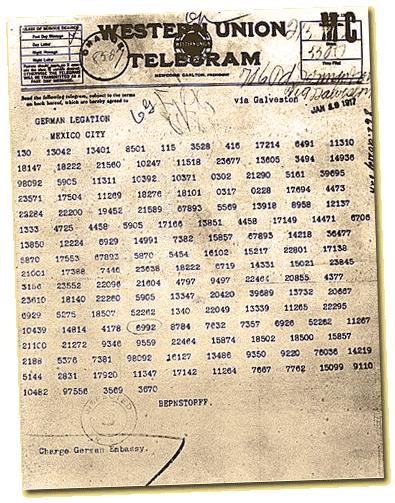
\includegraphics[width=0.8\linewidth]{zimmermann}
\caption{Zimmermann Note}
\end{figure}

This message is encrypted with a cipher named ``cipher 0075'', which is of course much more complicated than a simple substitution cipher. Yet the British had a crack team of codebreakers throughout both World Wars – known as Room 40 – and were able to apply more advanced versions of the techniques we saw above in order to break the cipher. When the Germans' clandestine proposal was revealed, Americans were outraged; this is viewed as one of the major tipping points that pulled the United States into World War I.

%% \bibliography{citations}
%% \bibliographystyle{ieeetr}

\end{CJK}
\end{document}
